%%%%%%%% ICML 2023 EXAMPLE LATEX SUBMISSION FILE %%%%%%%%%%%%%%%%%

\documentclass[nohyperref]{article}

% Recommended, but optional, packages for figures and better typesetting:
\usepackage{microtype}
\usepackage{graphicx}
\usepackage{subfigure}
\usepackage{booktabs} % for professional tables

% hyperref makes hyperlinks in the resulting PDF.
% If your build breaks (sometimes temporarily if a hyperlink spans a page)
% please comment out the following usepackage line and replace
% \usepackage{icml2023} with \usepackage[nohyperref]{icml2023} above.
\usepackage{hyperref}

\newlength{\bibitemsep}\setlength{\bibitemsep}{.2\baselineskip plus .05\baselineskip minus .05\baselineskip}
\newlength{\bibparskip}\setlength{\bibparskip}{0pt}
\let\oldthebibliography\thebibliography
\renewcommand\thebibliography[1]{%
  \oldthebibliography{#1}%
  \setlength{\parskip}{\bibitemsep}%
  \setlength{\itemsep}{\bibparskip}%
}

% Attempt to make hyperref and algorithmic work together better:
\newcommand{\theHalgorithm}{\arabic{algorithm}}

% Use the following line for the initial blind version submitted for review:
\usepackage[accepted]{icml2023}

% If accepted, instead use the following line for the camera-ready submission:
% \usepackage[accepted]{icml2022}

% For theorems and such
\usepackage{amsmath}
\usepackage{amssymb}
\usepackage{mathtools}
\usepackage{amsthm}

% if you use cleveref..
\usepackage[capitalize,noabbrev]{cleveref}

%%%%%%%%%%%%%%%%%%%%%%%%%%%%%%%%
% THEOREMS
%%%%%%%%%%%%%%%%%%%%%%%%%%%%%%%%
\theoremstyle{plain}
\newtheorem{theorem}{Theorem}[section]
\newtheorem{proposition}[theorem]{Proposition}
\newtheorem{lemma}[theorem]{Lemma}
\newtheorem{corollary}[theorem]{Corollary}
\theoremstyle{definition}
\newtheorem{definition}[theorem]{Definition}
\newtheorem{assumption}[theorem]{Assumption}
\theoremstyle{remark}
\newtheorem{remark}[theorem]{Remark}

% Todonotes is useful during development; simply uncomment the next line
%    and comment out the line below the next line to turn off comments
%\usepackage[disable,textsize=tiny]{todonotes}
\usepackage[textsize=tiny]{todonotes}


% The \icmltitle you define below is probably too long as a header.
% Therefore, a short form for the running title is supplied here:
\icmltitlerunning{SL Project}

\newcommand{\dnl}{\mbox{}\par}
\newcommand{\mycomment}[1]{\textbf{Note:} \textit{#1}}
\newcommand{\cnote}[1]{\textsf{\color{blue} [#1]}}
%\newcommand{\cnote}[1]{}


\begin{document}

\twocolumn[
\icmltitle{CS5033 - SL Project}

% It is OKAY to include author information, even for blind
% submissions: the style file will automatically remove it for you
% unless you've provided the [accepted] option to the icml2022
% package.

% List of affiliations: The first argument should be a (short)
% identifier you will use later to specify author affiliations
% Academic affiliations should list Department, University, City, Region, Country
% Industry affiliations should list Company, City, Region, Country

% You can specify symbols, otherwise they are numbered in order.
% Ideally, you should not use this facility. Affiliations will be numbered
% in order of appearance and this is the preferred way.
\icmlsetsymbol{equal}{*}

\begin{icmlauthorlist}
\icmlauthor{Airi Shimamura}{} %{equal,yyy}
\icmlauthor{Khoi Trinh}{} %{equal,yyy,comp}
%\icmlauthor{Firstname3 Lastname3}{comp}
%\icmlauthor{Firstname4 Lastname4}{sch}
%\icmlauthor{Firstname5 Lastname5}{yyy}
%\icmlauthor{Firstname6 Lastname6}{sch,yyy,comp}
%\icmlauthor{Firstname7 Lastname7}{comp}
%\icmlauthor{}{sch}
%\icmlauthor{Firstname8 Lastname8}{sch}
%\icmlauthor{Firstname8 Lastname8}{yyy,comp}
%\icmlauthor{}{sch}
%\icmlauthor{}{sch}
\end{icmlauthorlist}

%\icmlaffiliation{yyy}{Department of XXX, University of YYY, Location, Country}
%\icmlaffiliation{comp}{Company Name, Location, Country}
%\icmlaffiliation{sch}{School of ZZZ, Institute of WWW, Location, Country}

%\icmlcorrespondingauthor{Amy McGovern}{first1.last1@xxx.edu}
%\icmlcorrespondingauthor{Anna Partner}{first2.last2@www.uk}

% You may provide any keywords that you
% find helpful for describing your paper; these are used to populate
% the "keywords" metadata in the PDF but will not be shown in the document
%\icmlkeywords{Machine Learning, ICML}

\vskip 0.3in
]

% this must go after the closing bracket ] following \twocolumn[ ...

% This command actually creates the footnote in the first column
% listing the affiliations and the copyright notice.
% The command takes one argument, which is text to display at the start of the footnote.
% The \icmlEqualContribution command is standard text for equal contribution.
% Remove it (just {}) if you do not need this facility.

%\printAffiliationsAndNotice{}  % leave blank if no need to mention equal contribution
%\printAffiliationsAndNotice{\icmlEqualContribution} % otherwise use the standard text.

\section{Introduction}

For our Supervised Learning project this semester, we want to create a few models to predict a user's preference for a song on the Spotify streaming platform.

Each song on Spotify has their own set of 11 features. These features are: danceability, energy, key, loudness, mode, speechiness, acousticness, instrumentalness, liveness, valence, and tempo.

A user can request their streaming history from Spotify via the Privacy section of their account. For the purpose of this project, Khoi's one-year streaming history from February 2022 
to February 2023 will be used as the 1 class, for songs we like; and about 4200 random songs which Khoi has never heard will be used as the 0 class, for songs we do not like.

The dataset has 56,210 songs in class 1, and 4,170 songs in class 0. However, the songs in class 1 have duplicates, due to the nature of streaming a song multiple times, these will be removed.

For this project; Khoi implemented Logistic Regression, and Decision Trees; Airi implemented Naive Bayes, and Random Forest. We also compared our models with existing models from the scikit-learn package; namely Ridge Regression, Stochastic Gradient Descent, K-Nearest Neighbors, and Support Vector Machines.

\section{Overview and Preliminary Analysis}

One thing we wanted to explore from the data, is how the points are related to one another, through principal component analysis, and clustering. Using k-means clustering, with $k = 3$, we obtained the following figure.

Principal Component Analysis (PCA) is a technique in statistics and data analysis for reducing the dimensions of a dataset, finding patterns, and visualizing relationships. It works by identifying the principal components that explain the most variation in the data, and projecting the data onto these components. Several sources validate the effectiveness of PCA in various applications, such as genetics, finance, image processing, and ecology. Some notable references include the works of \cite{jolliffe2002principal}, \cite{hotelling1933analysis}, and \cite{pearson1901lines}. We were able to reduce our numeric features into 2 principal components.

Looking at the Figure 1, we can see that Principal Component 1 separate songs with higher liveness, speechiness, and loudness, and those with lower danceability and energy (these mostly belong to Cluster 0 and 2), and Principal Component 2 separate songs with higher instrumentalness, loudness, and those with lower acousticness (these mostly belong to Cluster 2). Overall, we can see that Cluster 0 has songs that are higher in loudness, speechiness, and liveness. Cluster 1 has songs that are lower in danceability and energy. Cluster 2 has songs high in speechiness, liveness, acousticness, but lower in instrumentalness.

\section{Hypotheses}
Our \textbf{first hypothesis} is that our supervised learning models will be able to classify these songs as likes or dislikes with at least 90\% accuracy.

Our \textbf{second hypothesis} is that out of the four chosen algorithms; Random Forest will give us the best performance; followed by Decision Tree, then Logistic Regression, and finally Naive Bayes. We will evaluate each algorithm's performance by first comparing the Accuracy value, then the values of Precision, Recall, and produce ROC curves for each algorithm, should the accuracy be equal.

\section{Experimental Results and Analysis}

\subsection{Khoi's Experiments}

For this project, Khoi implemented logistic regression and decision tree.

\textbf{Logistic Regression} is a statistical machine learning algorithm predicting the probability of a target variable by fitting a logistic function to the input features. This optimizes the parameters of the logistic function by minimizing the cost function, which measures the difference between the predicted probabilities and the actual class labels.

For this model, Khoi implemented the following functions:

Sigmoid/Logistic function: $\sigma(z) = \frac{1}{1 + e^{-z}}$

% j = -1/m * (y.T.dot(np.log(h + eps)) + (1-y).T.dot(np.log(1-h + eps)))
Logistic loss function: $log loss = \Sigma_{x, y \in D} -ylog(y') - (1 - y)log(1 - y')$

Where:

$(x, y) \in D$ is the data set containing labeled instances.

$y$ is the label in a labeled example; in this case, it is either 0 or 1.

$y'$ is the predicted value, given the features in x.

Khoi also implemented the logistic regression function from scratch, and can be seen in the code provided.

\textbf{Decision Tree} is a machine learning algorithm used to predict the class of an input based on its features. This algorithm partitions the input space into increasingly smaller regions based on the values of the input features by selecting the features and test conditions that best separate the training data into the different classes. This process is repeated recursively to create a tree-like structure until a final decision is made.

Similar to the previous model, Khoi implemented this from scratch, and can be seen in the provided code. The criteria Khoi is using to split the node is the Gini impurity. This is a measure of the impurity or randomness of a set of examples used in decision trees. It measures the probability that two randomly chosen examples from the set have different class labels. The aim is to find the split that results in the lowest Gini impurity of the resulting subsets. With that being said, in \cite{breiman1984classification}, the author mentioned that decision tree can achieve high accuracy, but can be unstable due to small changes in the training data.

The results for these algorithms will be included in table 1.

\subsection{Airi's Experiments}

Airi implemented Naive Bayes and Random Forest algorithms.

\textbf{Naive Bayes} is a group of probabilistic machine learning algorithms based on applying Bayes’ theorem with the assumption of independence between features. This assumes that the presence or absence of one feature does not affect the presence or absence of any other feature within a class, and calculates the probabilities of each class label given the values of the features from the input. The class with the highest probability is then selected as the predicted class label for the given input. In a study conducted by \cite{singh2017impact}, it is stated that Naive Bayes performed better on nominal data, while its performance on numerical and mixed data was dropped. Te majority of our data is numerical, meaning the performance of our model was not as good as other models such as K-NN or Random Forest as shown in table 1. 

\textbf{Random Forest} is an ensemble learning method that combines multiple decision trees to improve performance and reduce over-fitting. Airi was able to build her model based on Khoi's Decision Tree code. In a study conducted by \cite{tangirala2020evaluating}, it was found that both Gini impurity or Information gain provided similar performances regardless of whether the data set was balanced or unbalanced. However, the Gini index outperformed information gain in terms of accuracy on certain datasets, while information gain exhibited better computational time efficiency. 

In addition, according to \cite{singh2017impact}, Random Forest performed better on numerical data, while its performance dropped for nominal and mixed data. Even though our dataset is mixed data, our Random Forest model still achieved an accuracy of over 98\% .

For this model, Airi used the Gini index as the criterion for tree splitting, varying the number of decision trees from 10 to 100 with depth = 10 and selecting the best performance. The maximum accuracy was achieved when the number of trees was set to 30.

The results for these algorithms will be included in table 1.

\subsection{Hypothesis 1}

Table 1 shows our results.

\begin{table}[H]
\centering
\resizebox{\columnwidth}{!}{%
\begin{tabular}{lllll}
          & Log Reg & Naive Bayes & Decision Tree & Random Forest \\
Accuracy  & 97.6\%  & 97.45\%     & 98.07\%       & 98.61\%           \\
Precision & 96.19\% & 97.58\%     & 97.02\%       & 98.63\%           \\
Recall    & 97.22\% & 96.88\%     & 97.64         & 98.35\%     \\
Runtime(ms)    & 677.4   &65.41        & 12789.01      & 270066.1 
\end{tabular}%
}
\caption{\label{demo-table}Results Of Our Experiments}
%\vspace{-4mm}
\end{table}
\raggedbottom

From the above results, we can see that our experiments matched the expectations of hypothesis 1; all four of our models performed with accuracy better than 90\%.

\subsection{Hypothesis 2}

For this hypothesis, we first compared the accuracy of each algorithm, then the area under the curve (AUC), and finally, the running time. The algorithm with the higher accuracy is generally considered to be better. If the accuracy is the same, then a higher AUC indicates a better algorithm. Finally, if both accuracy and AUC are the same, then the faster algorithm is the better one. 

Looking at table 1, we can see that we only needed to compare accuracy. This means that Random Forest performed best, followed by Decision Tree, then Logistic Regression, and finally Naive Bayes.

Overall, the four algorithms were ranked as expected.


\section{Related Work Reviews}

We both compared our models with built-in models from the scikit-learn python package. Khoi compared Logistric Regression with Ridge Reggrsion, Decision Tree with Stochastic Gradient Descent.

\textbf{Ridge regression} is a regularized regression method that addresses the issue of overfitting by adding a penalty term to the loss function. According to \cite{hastie2009elements}, ridge regression can improve prediction accuracy when the number of predictor variables is large and highly correlated. With our dataset, ridge regression has similar, but slightly lower accuracy, however, it achieved higher precision, and lower recall when compared to Logistics Regression.

\textbf{Stochastic gradient descent (SGD)} is an iterative optimization algorithm commonly used for training neural networks and other machine learning models. Compared to batch gradient descent, which updates the model weights based on the entire training dataset, SGD updates the weights based on small batches of data, leading to faster convergence. In the paper by \cite{zhang2017understanding}, the author stated SGD can achieve higher accuracy and faster convergence compared to other optimization methods for deep learning. When compared to the current decision tree model (with depth 5), SGD performed worse, with lower accuracy, precision, and recall.

For Airi, she compared her models with K-Nearest Neighbors, and Support Vector Machine (SVM)

\textbf{K-nearest neighbors} is a non-parametric classification and regression method that uses the k-nearest data points in the training set to make predictions. In the research by \cite{cover1967nearest}, it was found that KNN can achieve high classification accuracy but may suffer from the curse of dimensionality when the number of predictors is high. Addtionally, the study by \cite{jadhav2016comparative} found that K-NN performed better on datasets with smaller numbers of features and larger numbers of instances. Finally, according to \cite{singh2017impact}, K-NN performed better on mixed data, while its performances dropped on numerical and nominal data.

Our dataset has only 11 features and a large number of instances, consisting of both numerical and categorical data, our K-NN model performed better than Naive Bayes but did not reach the level of performance achieved by the Random Forest model.

In Airi's case, she compared K-NN model with different numbers of the nearest neighbors from 1 to 100 and obtain the best number of k value.

\textbf{Support vector machines (SVM)} are popular supervised learning methods that seeks to find the hyperplane that maximally separates the different classes in the input space. \cite{cortes1995support} stated that SVM can achieve higher classification accuracy than other methods such as neural networks and decision trees, especially in high-dimensional spaces.

With our data, SVM performed worse than Random Forest, with a lower accuracy, precision, and recall.

Table 2 shows the results of these scikit-learn models:

% Please add the following required packages to your document preamble:
% \usepackage{graphicx}
\begin{table}[H]
\centering
\resizebox{\columnwidth}{!}{%
\begin{tabular}{lllll}
          & Ridge Reg & SGD & KNN & SVM \\
Accuracy  & 97.29\%  & 97.6\%     & 98.14\%       & 97.83\%           \\
Precision & 97.16\% & 96.58\%     & 98.12\%       & 97.78\%           \\
Recall    & 95.29\% & 96.79\%     & 97.85\%       & 97.51\%  \\
\end{tabular}%
}
\caption{\label{demo-table}Comparison Models' Results}
%\vspace{-12mm}
\end{table}
\raggedbottom



\section{Conclusion and Future Work}

In conclusion, throughout the project, we were able to implement our own algorithms for predicting a user's preference for a particular song on Spotify. All of our algorithms achieved more than 90\% accuracy, and they were ranked as hypothesized; with Random Forest performing best, followed by Decision Tree, Logistic Regression, and Naive Bayes.

In the future, we would like to implement these algorithms using a larger dataset. Spotify also allows users to request their lifetime streaming history, and in Khoi's case, this would result in a much larger dataset, as he has been using the platform for a while. Furthermore, we found that the performance of these algorithms varied depending on the type of data used through the research papers. The data set we used consists of mostly continuous variables, so we would like to find out how their performances change if we add more or remove categorical variables. 

\section{Relevant Figures}

This section includes any figures relevant to the project. It has the PCA results, and the ROC curves for our model, as well as a comparison of performance for the Random Forest algorithm

\begin{figure}[H] %h forces the figure to be inserted right here
    \centering
    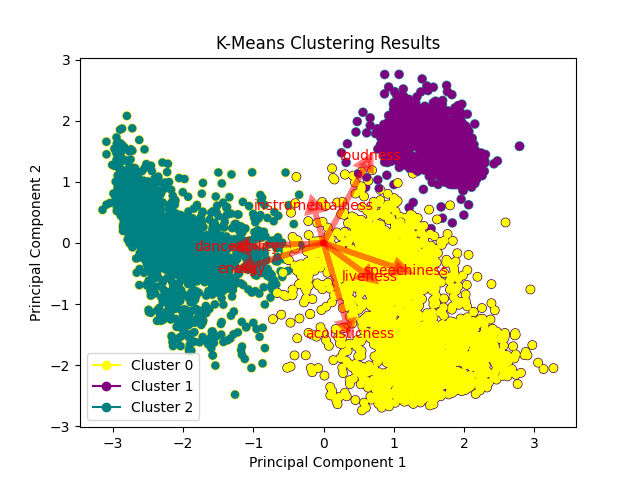
\includegraphics[width=0.75\linewidth]{figs/kmeanscluster.png}
    \caption{Clustering PCA Results}
    \vspace{-8mm}
\end{figure}

%Here are the ROC curves for the algorithms created for this project.

\begin{figure}[H] %h forces the figure to be inserted right here
    \centering
    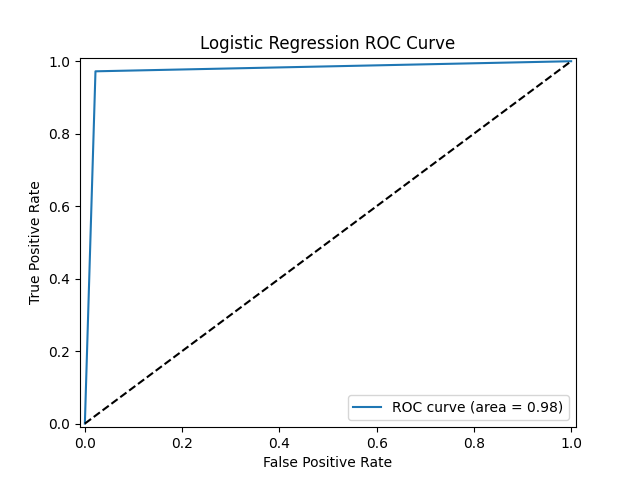
\includegraphics[width=0.75\linewidth]{figs/logistic-regressionROC.png}
    \caption{Logistic Regression ROC}
    \vspace{-8mm}
\end{figure}

\begin{figure}[H] %h forces the figure to be inserted right here
    \centering
    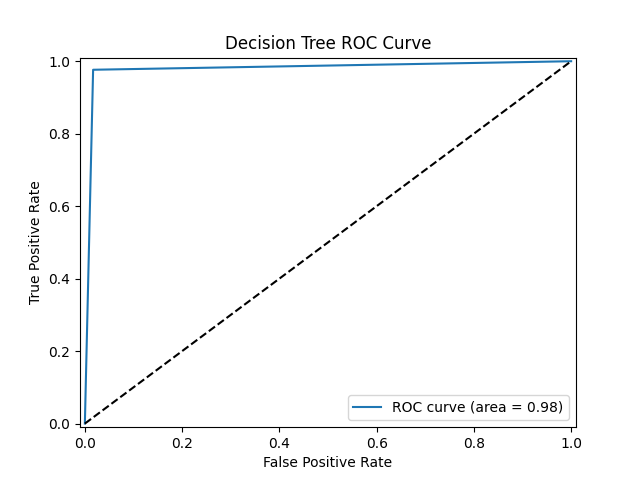
\includegraphics[width=0.75\linewidth]{figs/decision-treeROC.png}
    \caption{Decision Tree ROC}
    \vspace{-8mm}
\end{figure}

% \begin{figure}[H] %h forces the figure to be inserted right here
%     \centering
%     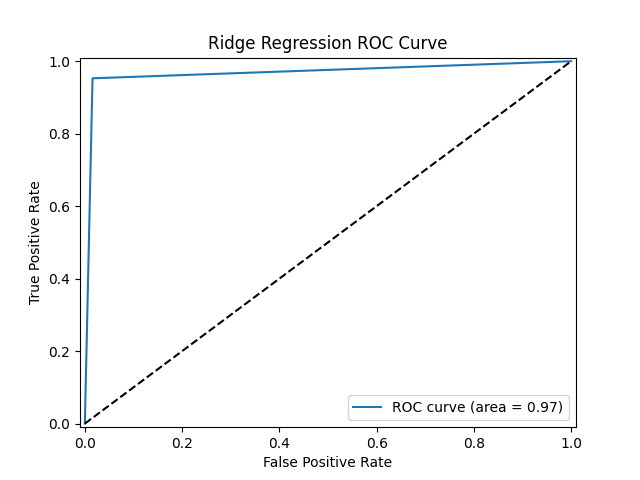
\includegraphics[width=0.75\linewidth]{figs/scikitridgeROC.png}
%     \caption{Ridge Regression ROC}
%     \vspace{-7mm}
% \end{figure}

% \begin{figure}[H] %h forces the figure to be inserted right here
%     \centering
%     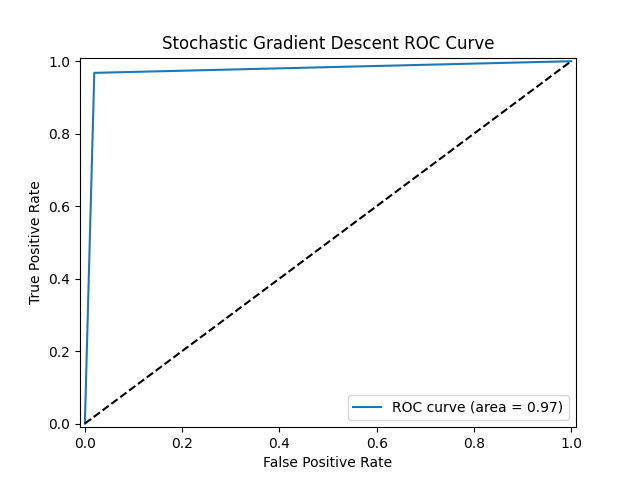
\includegraphics[width=0.75\linewidth]{figs/scikitSGD-ROC.png}
%     \caption{Stochastic Gradient Descent ROC}
%     \vspace{-4mm}
% \end{figure}

\begin{figure}[H] %h forces the figure to be inserted right here
    \centering
    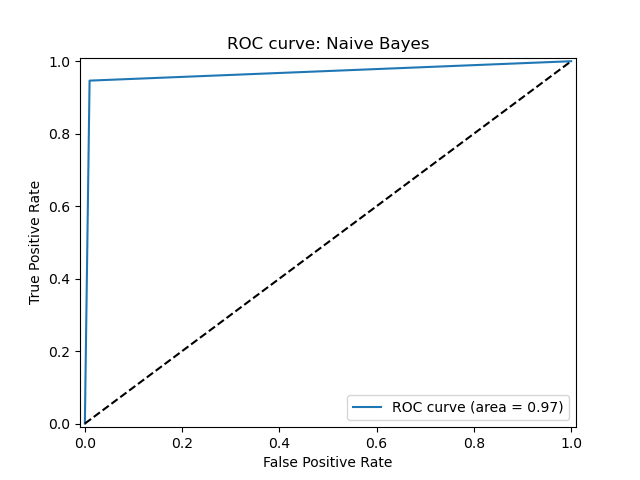
\includegraphics[width=0.75\linewidth]{figs/naive-bayes-ROC.png}
    \caption{Naive Bayes ROC}
    \vspace{-8mm}
\end{figure}

\begin{figure}[H] %h forces the figure to be inserted right here
    \centering
    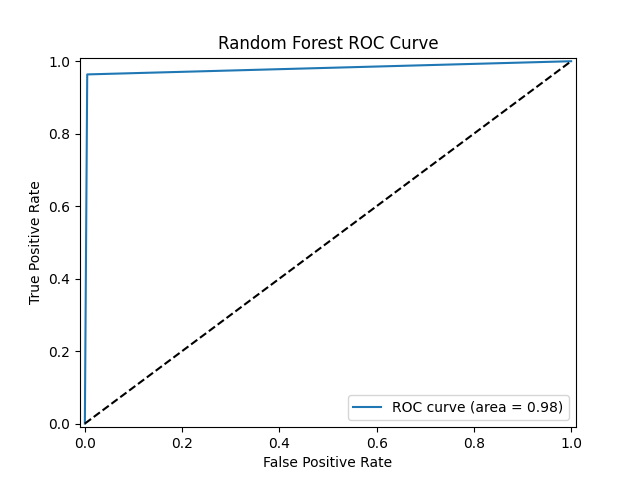
\includegraphics[width=0.75\linewidth]{figs/random-forest-ROC.png}
    \caption{Random Forest ROC}
    \vspace{-8mm}
\end{figure}

% \begin{figure}[H] %h forces the figure to be inserted right here
%     \centering
%     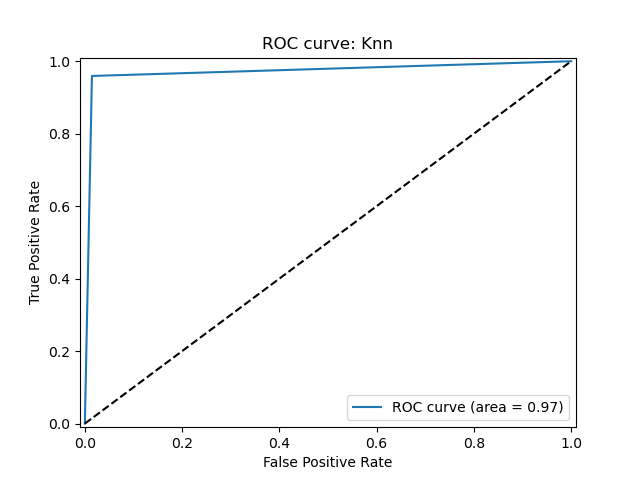
\includegraphics[width=0.75\linewidth]{figs/knn-ROC.png}
%     \caption{K-NN ROC}
%     \vspace{-4mm}
% \end{figure}

% \begin{figure}[H] %h forces the figure to be inserted right here
%     \centering
%     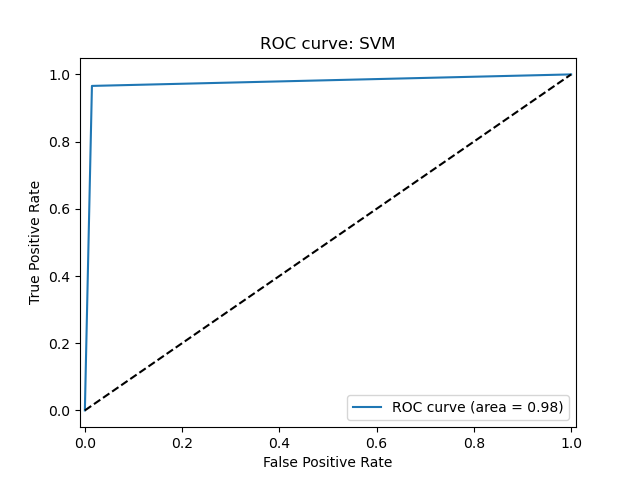
\includegraphics[width=0.75\linewidth]{figs/svm-ROC.png}
%     \caption{SVM ROC}
%     \vspace{-4mm}
% \end{figure}

%Here is the  Random Forest result with depth = 10, and number of trees from 10 to 100

\begin{figure}[H] %h forces the figure to be inserted right here
    \centering
    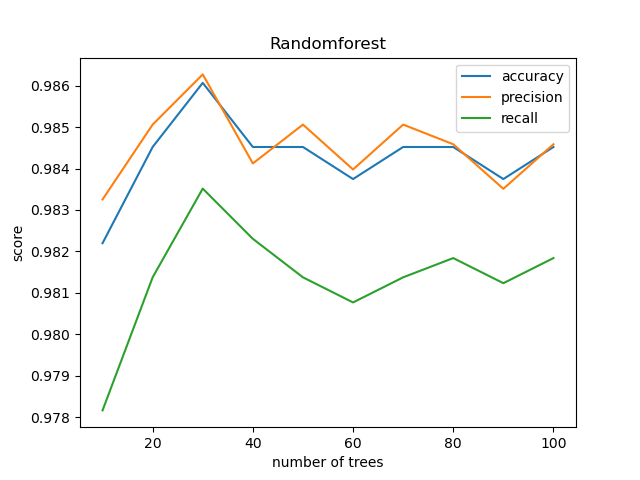
\includegraphics[width=0.75\linewidth]{figs/randomforest_scores(final).png}
    \caption{Result of Random Forest}
    \vspace{-7.5mm}
\end{figure}

% Here is the performance of K-NN with different number of neighbors from 1 to 100 

% \begin{figure}[H] %h forces the figure to be inserted right here
%     \centering
%     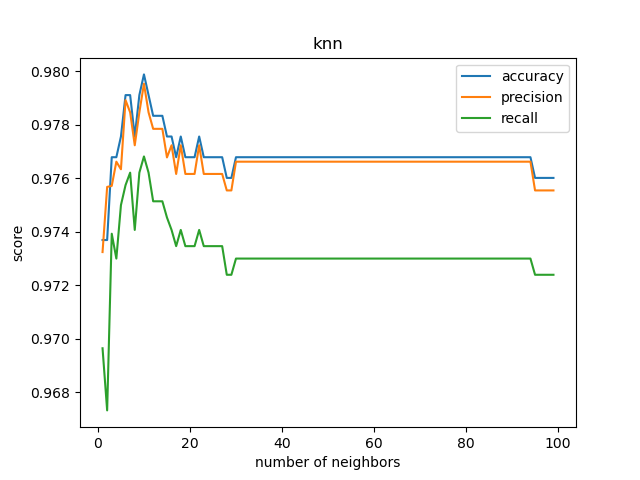
\includegraphics[width=0.75\linewidth]{figs/knn_scores.png}
%     \caption{Result of K-NN}
%     \vspace{-7mm}
% \end{figure}


%\cnote{All written proposals must be no longer than one page per number of people in the group.}


\bibliographystyle{mslapa}
\bibliography{ref.bib}

\end{document}


% This document was modified from the file originally made available by
% Pat Langley and Andrea Danyluk for ICML-2K. This version was created
% by Iain Murray in 2018, and modified by Alexandre Bouchard in
% 2019 and 2021 and by Csaba Szepesvari, Gang Niu and Sivan Sabato in 2022. 
% Previous contributors include Dan Roy, Lise Getoor and Tobias
% Scheffer, which was slightly modified from the 2010 version by
% Thorsten Joachims & Johannes Fuernkranz, slightly modified from the
% 2009 version by Kiri Wagstaff and Sam Roweis's 2008 version, which is
% slightly modified from Prasad Tadepalli's 2007 version which is a
% lightly changed version of the previous year's version by Andrew
% Moore, which was in turn edited from those of Kristian Kersting and
% Codrina Lauth. Alex Smola contributed to the algorithmic style files.
